
% This LaTeX was auto-generated from MATLAB code.
% To make changes, update the MATLAB code and republish this document.

\documentclass[a4paper]{article}
\usepackage{graphicx}
\usepackage{color}
\usepackage{amsmath}
\usepackage{pdfpages}

\sloppy
\definecolor{lightgray}{gray}{0.5}
\setlength{\parindent}{0pt}

\begin{document}

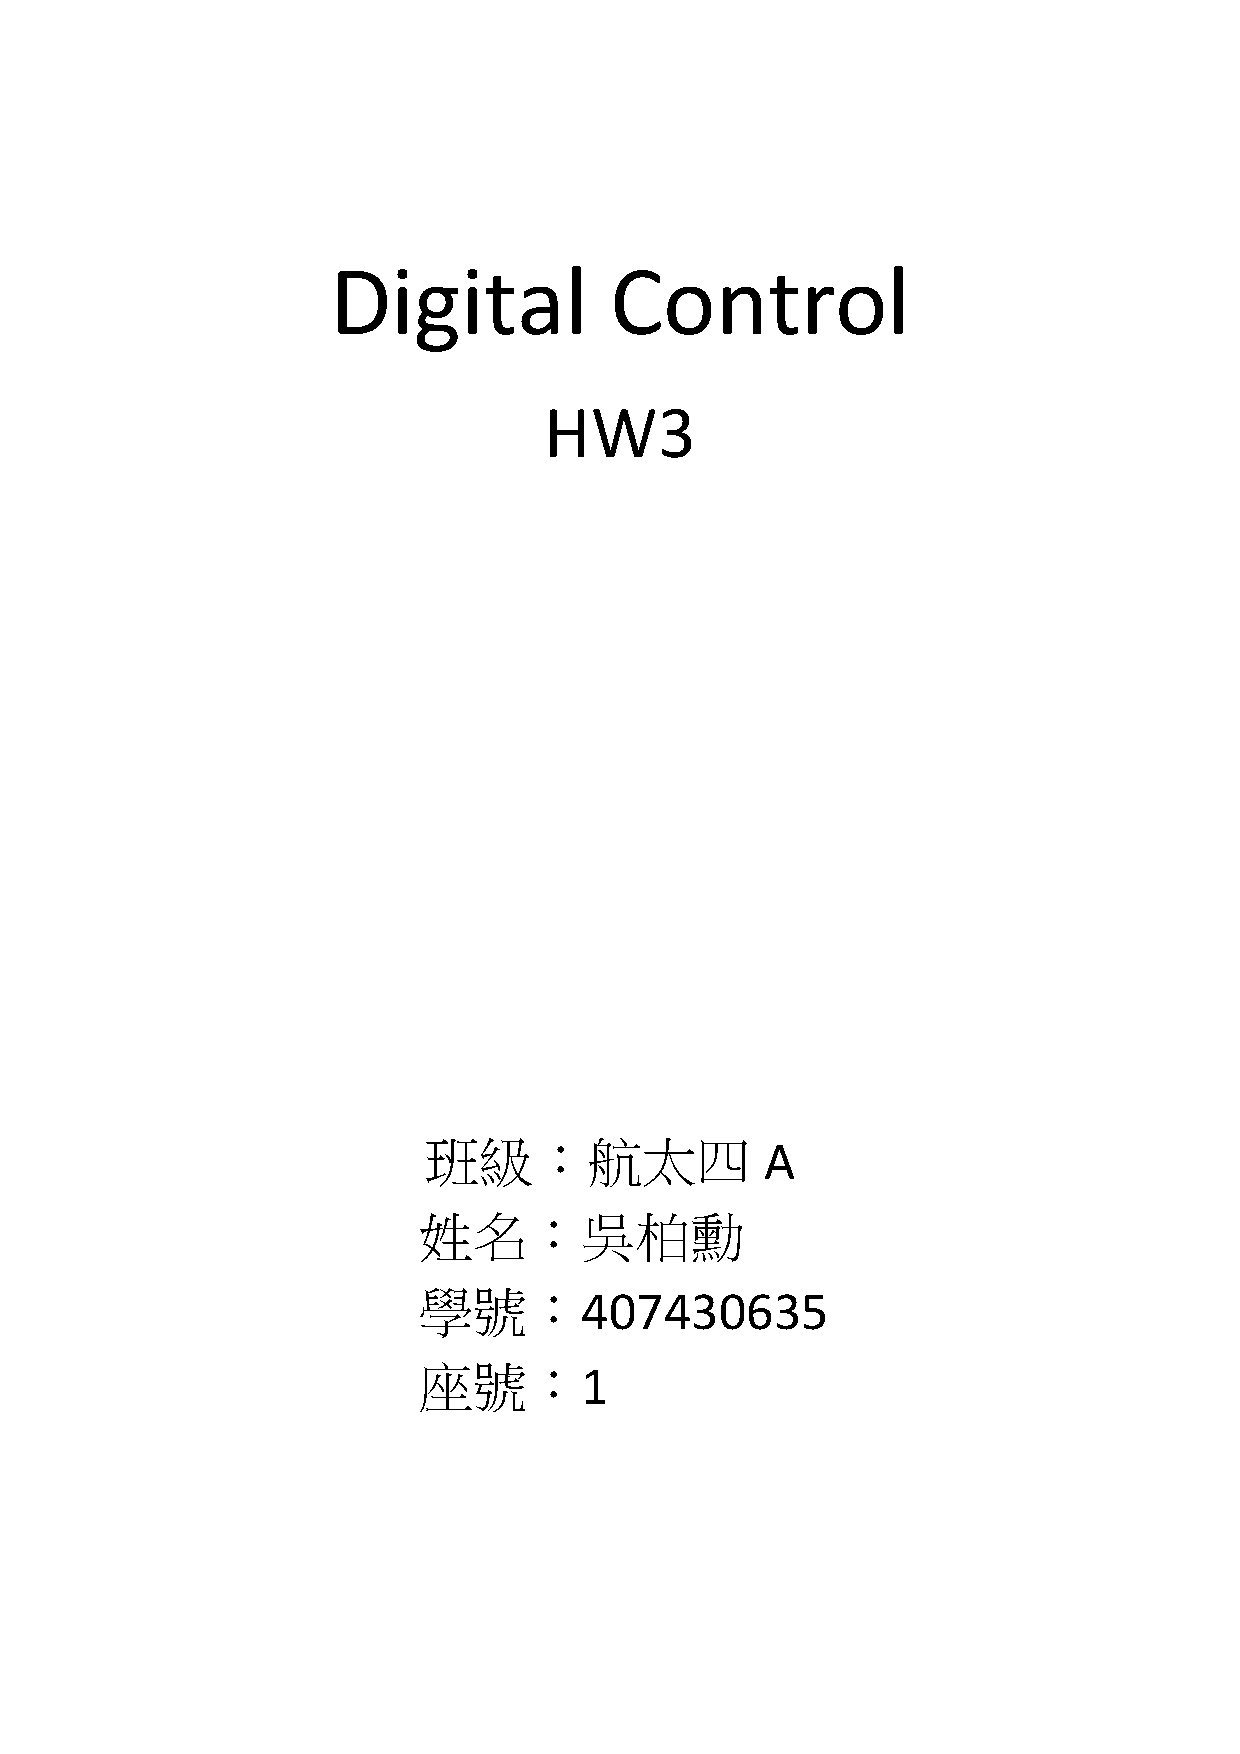
\includepdf[]{../數位控制封面.pdf}

\subsection*{\#1}

\begin{par}
    Let $r=k+2$, then
    \begin{equation}x(r)-1.3x(r-1)+0.4x(r-2)=u(r-2)\end{equation}
    and the condition of system was
    \begin{equation}x(k)=0, \quad for \ r=0,1\end{equation}
    \begin{equation}
        u(r)=
        \begin{cases}
            0, \quad r<2\\
            1, \quad r\geq2
        \end{cases}
    \end{equation}
\end{par}
\hrulefill

\begin{verbatim}
clear;clc;close all
x = [0 0];
k2r = @(k) k+2;
for k = 0:100
    if k2r(k-2) >= 2
        u = 1;
    else
        u = 0;
    end
    x(k2r(k)+1) = 1.3*x(k2r(k-1)+1)-0.4*x(k2r(k-2)+1)+u;
end
plot(1:length(x)-2,x(3:end))
grid()
xlabel("k")
ylabel("x")
\end{verbatim}

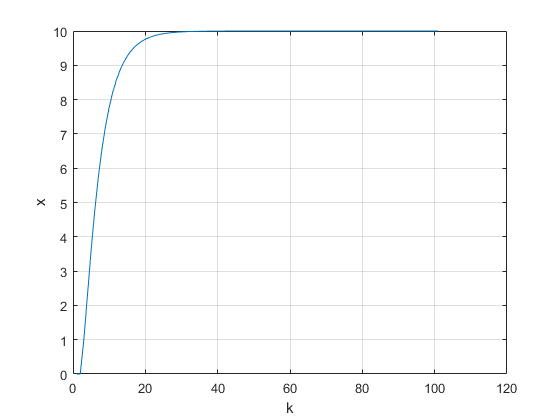
\includegraphics [width=4in]{HW3_01.png}



\end{document}

